\title{Final for Calculus-Based Physics: Electricity and Magnetism}
\author{Dr. Jordan Hanson - Whittier College Dept. of Physics and Astronomy}
\date{\today}
\documentclass[10pt]{article}
\usepackage[a4paper, total={18cm, 27cm}]{geometry}
\usepackage{outlines}
\usepackage{graphicx}
\usepackage{amsmath}
\begin{document}
\maketitle

\section{Equations and constants}

\begin{enumerate}
\item Volume of a sphere: $V_s = \frac{4}{3}\pi r^3$.
\item Density, mass and volume: $m = \rho V$.
\item Charge density, charge and volume: $Q = \rho V$.
\item Coulomb force: $\vec{F}_C = k \frac{q_1 q_2}{r^2}\hat{r}$.
\item Definition of electric field: $\vec{F}_C = q\vec{E}$.
\item Definition of electric flux: $\phi_E = \vec{E} \cdot \vec{A}$.
\item Gauss' Law: $\phi_E = q_{enc}/\epsilon_0$. (Assumes field is uniform over the surface).
\item Voltage and electric field, one dimension, uniform field: $|E| = - \frac{\Delta V}{\Delta x}$.
\item Voltage and electric field, general case: $\vec{E} = -\nabla V$.
\item Ohm's Law: $V = IR$.
\item Electrical power: $P = IV = I^2 R = V^2/R$.
\item Magnetic dipole moment: $\vec{\mu} = I \vec{A}$, where $\vec{A}$ is the area vector.
\item Torque on a magnetic dipole: $\tau = \vec{\mu} \times \vec{B}$.
\item Definition of magnetic flux: $\phi_m = \vec{B} \cdot \vec{A}$.  The units are T m$^2$, which is called a Weber, or Wb.
\item Faraday's Law: $emf = -N \frac{d \phi}{d t}$
\item Faraday's Law using \textbf{Inductance}, M: $emf = -M \frac{dI}{dt}$.
\item Typically, we refer to \textit{mutual inductance} between two objects as $M$, and \textit{self inductance} as $L$.
\item Inductance of a solenoid: $L = \mu_0 n^2 V$
\item Magnetic permeability: $\mu_0 = 4\pi \times 10^{-7}$ T m A$^{-1}$
\item Units of inductance: V s A$^{-1}$, which is called a Henry, or H.
\item Coulomb constant: $k = 8.9876 \times 10^{9}$ N m$^2$ C$^{-2}$.
\item Fundamental charge: $q_e = 1.602 \times 10^{-19}$ C.
\end{enumerate}

\clearpage

\section{Exercises}

\begin{enumerate}
\item \textbf{Chapters 5-6: Electrostatics and Gauss' Law}
\begin{enumerate}
\item A spherical water droplet of radius $25 \times 10^{-6}$ m carries an excess of 250 electrons.  The density of water is 997 kg m$^{-3}$.  (a) Calculate the mass of the water droplet. (b) Second, work out the total excess charge of the water droplet.  (c) What is the electric field required to balance the force of gravity on the drop? (d) Write an expression for the electric field outside of the water droplet assuming it is a sphere.  \\ \vspace{3.5cm}
%\item Two non-conducting spheres are uniformly charged with charges $Q_1$ and $Q_2$, respectively.  The geometry of the system is depicted in Fig. \ref{fig:spheres}.  (a) Using Gauss' law, write the expression for the electric field of each sphere separately, observed at $P$ for each.  (b) Sum the total electric field due to spheres 1 and 2, observed at point $P$, for $\theta = 45$ deg, $Q_1 = Q_2 = 1.0$ $\mu$C, and $r = 1.0$ m. \\ \vspace{3.5cm}
%\begin{figure}
%\centering
%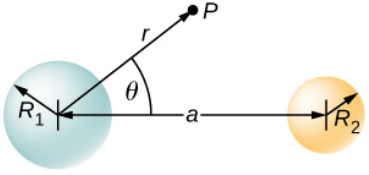
\includegraphics[width=0.3\textwidth]{spheres.png}
%\caption{\label{fig:spheres} Two charged spheres with radii $R_1$ and $R_2$, separated by a distance $a$, observed at a point $P$ at a distance $r$ from the center of sphere 1, at an angle $\theta$ with respect to the line between the spheres.  Assume that $P$ is also a distance $r$ from sphere 2.}
%\end{figure}
\end{enumerate}
\item \textbf{Chapters 7-8: Voltage and Capacitance}
\begin{enumerate}
\item The voltage across a membrane forming a cell wall is 80.0 mV and the membrane is 9.00 nm thick. What is the electric field strength? (The value is surprisingly large, but correct.) You may assume a uniform electric field. \\ \vspace{2cm}
\item An electric potential is defined by $V(x,y,z) = a x^2 + b y^2 + c z^2$, with $a = 2.0$ V m$^{-2}$, $b = 1.0$ V m$^{-2}$, and $c = 4.0$ V m$^{-2}$.  What is the corresponding electric field at $P = (0,1,1)$? \\ \vspace{3.5cm}
\end{enumerate}
\item \textbf{Chapters 9-10: Current, Resistance, and DC Circuits}
\begin{enumerate}
\item
\begin{figure}
\centering
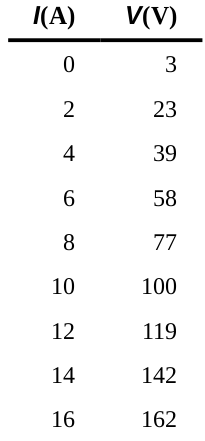
\includegraphics[width=0.12\textwidth]{OhmsTable.png}
\caption{\label{fig:OhmsTable} A table of current (left column) and voltage (right column) data for a sample of material.}
\end{figure} 
Figure \ref{fig:OhmsTable} contains the measurements of a current through and the voltage across a sample of material. Plot at least three data points in a graph below, and estimate the resistance. \\ \vspace{3cm}
\item An alternative to CFL bulbs and incandescent bulbs are light-emitting diode (LED) bulbs. A 100-W incandescent bulb can be replaced by a 16-W LED bulb.  Both produce 1600 lumens of light. Assuming the cost of electricity is \$0.10 per kilowatt-hour, how much does it cost to run the bulb for one year if it runs for four hours a day? \\ \vspace{2cm}
\item Two AA batteries are connected \textit{in parallel} with a load resistor $R$, as shown in Fig. \ref{fig:batt1} (left).  The two internal resistances are $r_1$ and $r_2$, and the two emf's are $\mathcal{E}_1$ and $\mathcal{E}_2$. Assume $r_1 = r_2$ and $\mathcal{E}_1 = \mathcal{E}_2$.  (a) Using the junction rule once, and the loop rule twice, solve for the current through the load resistor algebraically. (b) If  $\mathcal{E}_1 = \mathcal{E}_2 = 1.5$ V, $r_1 = r_2 = 0.1 \Omega$, and $R = 100\Omega$, what is the current through $R$? \\ \vspace{4cm}
\begin{figure}
\centering
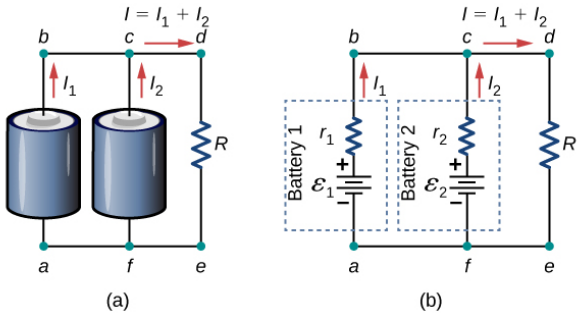
\includegraphics[width=0.4\textwidth]{batt1.png}
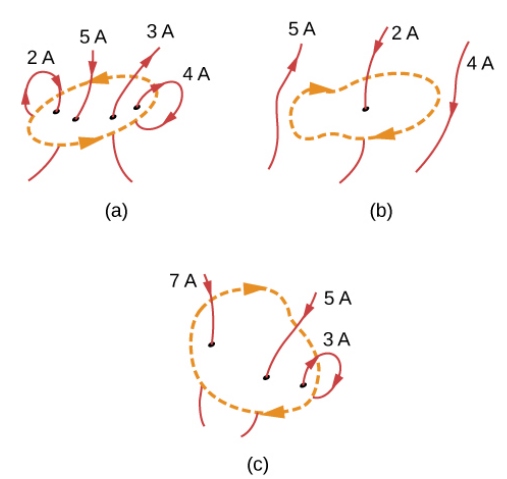
\includegraphics[width=0.3\textwidth]{amplaw.png}
\caption{\label{fig:batt1} (Left) Two batteries (a) connected in parallel with internal resistances can be modelled by a circuit (b). (Right) Three configurations of currents and loops.}
\end{figure}
\end{enumerate}
\item \textbf{Chapters 11-12: Magnetic fields and Sources of Magnetic Fields}
\begin{enumerate}
\item A circular loop of wire of area $10^{-2}$ m$^{2}$ carries a current of 20.0 A.  At a particular instant, the loop lies in the $xy$-plane and is subjected to a magnetic field $\vec{B} = \left( 3.0 \hat{i} + 6.0 \hat{j} + 3.0 \hat{k} \right) \times 10^{-2}$ T.  As
viewed from above the xy-plane, the current is circulating clockwise. (a) What is the magnetic dipole moment of the current loop? (b) At this instant, what is the magnetic torque on the loop? \\ \vspace{3cm}
\item
Use Amp\`{e}re's Law to evaluate $\oint \vec{B} \cdot d\vec{l}$ for the current configurations and paths (a)-(c) in Fig. \ref{fig:batt1} (right). \\ \vspace{2cm}
\end{enumerate}
\item \textbf{Chapters 13-14: Electromagnetic Induction and Inductance}
\begin{enumerate}
\item 
\begin{figure}
\centering
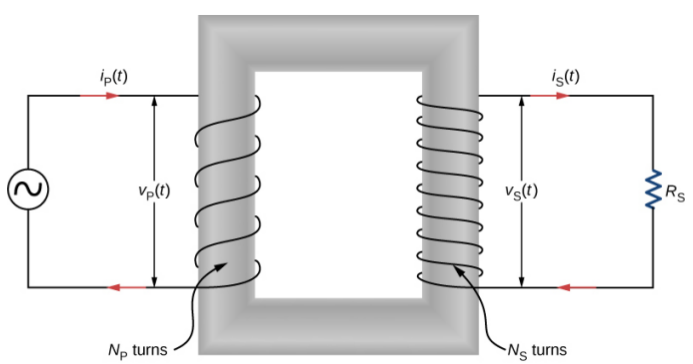
\includegraphics[width=0.45\textwidth]{transformer.png}
\caption{\label{fig:trans} The basic diagram for a \textit{transformer}...No, not Megatron the thing that gives us AC power.}
\end{figure}
In Fig. \ref{fig:trans} (left) a \textit{transformer} is depicted.  The gray square represents an iron core which ensures that the magnitude of the magnetic flux through the left solenoid \textbf{is identical to} the magnetic flux on the right solenoid.  Both solenoids are $L = 5$ cm long.  Suppose the left solenoid has $N_L = 500$ turns, and the right solenoid has $N_R = 1000$ turns.  Let the induced emf in the left solenoid be $v_L$, and the induced emf in the right solenoid be $v_R$.  Show that
\begin{equation}
\frac{v_L}{N_L} = \frac{v_R}{N_R}
\end{equation} \\ \vspace{3cm}
\item The two solenoids in Fig. \ref{fig:trans} each have volume $V = 5 \times 10^{-6}$ m$^3$, and length $l = 1.0$ cm.  What is the inductance of each, in Henries? \\ \vspace{3cm}
\item Suppose the current changes in the left solenoid of Fig. \ref{fig:trans} at a rate of 100 A s$^{-1}$.  (a) Using the inductance of the left solenoid, what is the induced emf in the left solenoid? (b) Using the result that $\frac{v_L}{N_L} = \frac{v_R}{N_R}$, calculate the induced emf in the right solenoid. \\ \vspace{4cm}
\end{enumerate}
\end{enumerate}

\end{document}